%
% Sección de clasificación de algoritmos tokenizadores,
% presentación de TT 1.
%
% Proyecto Lovelace.
%

\subsection{Clasificación}

\begin{frame}{Clasificación del PCI SSC}

  \begin{figure}[H]
    \begin{center}
      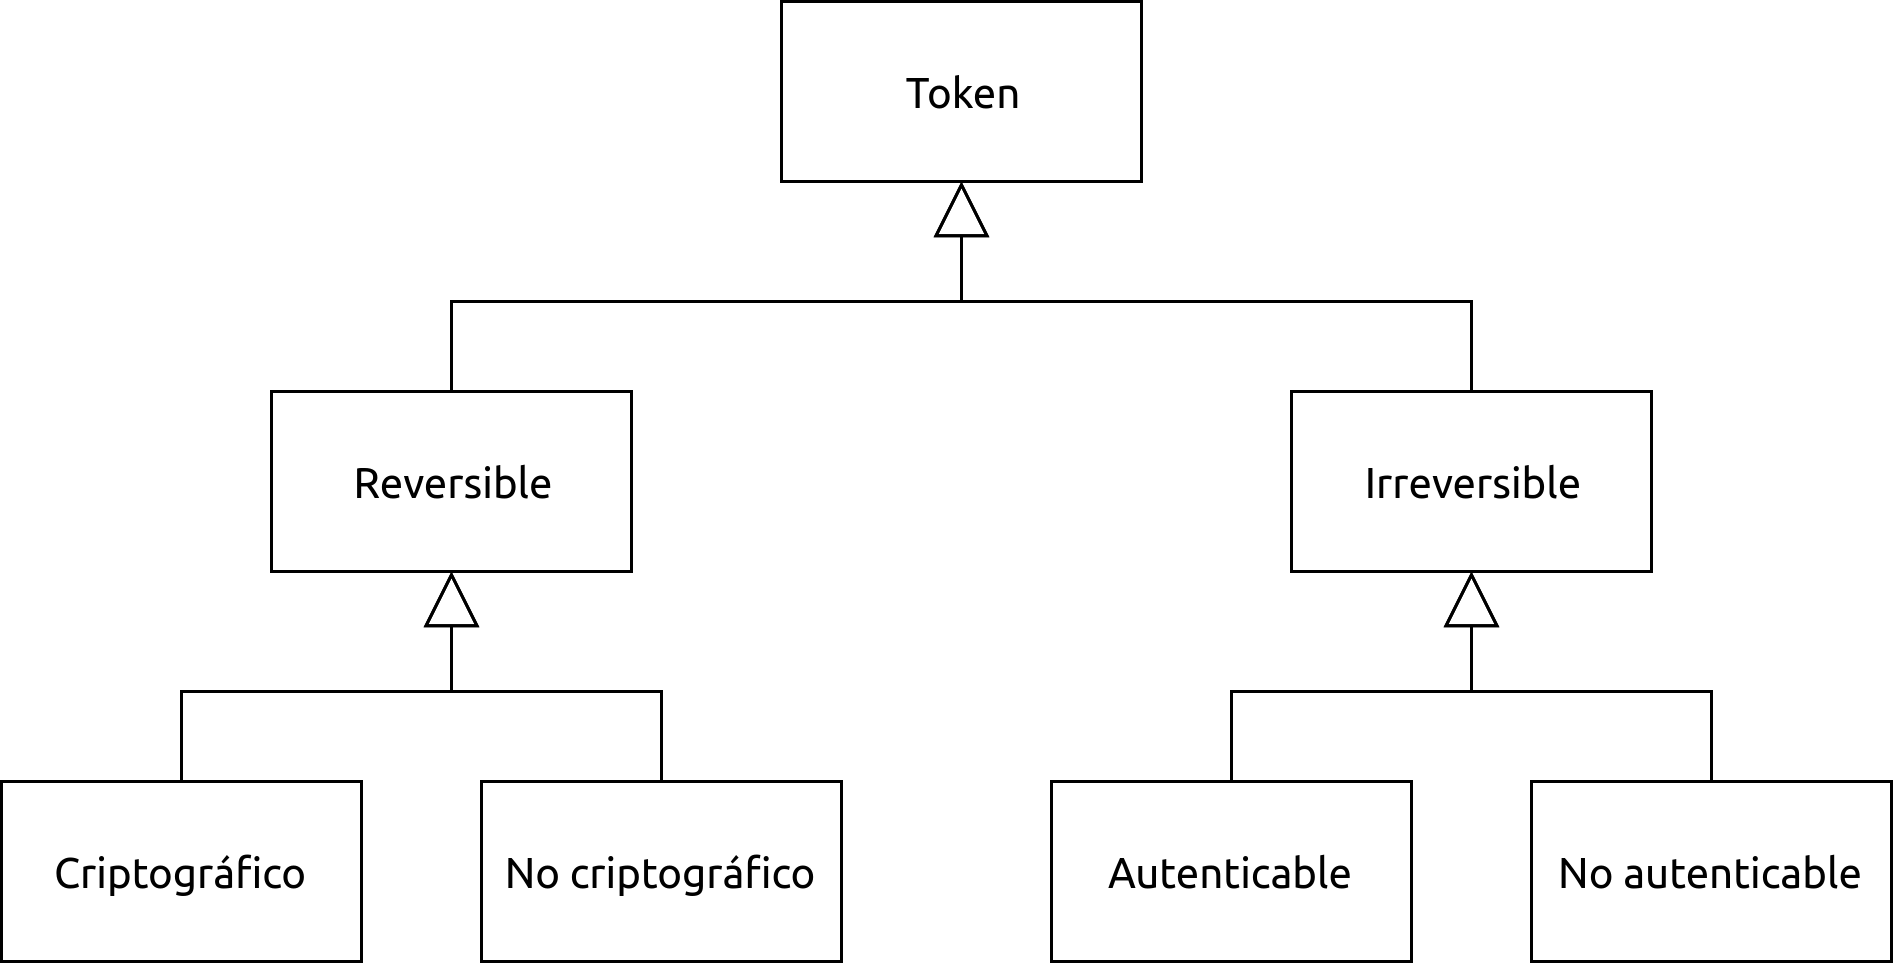
\includegraphics[width=1.0\linewidth]
        {../../../diagramas_comunes/clasificacion/clasificacion.png}
      \caption{Clasificación de \textit{tokens}~\cite{pci_tokens}.}
    \end{center}
  \end{figure}

  \note
  {
    Los irreversibles no pueden ser reconvertidos al PAN (de ninguna manera,
    mas que con fuerza bruta). Los autenticables funcionan como una función
    Hash: si tienes el PAN y el token, se puede validar que ese token es el
    par de ese PAN. Los no autenticables no pueden validar esto último.

    Los reversibles permiten obtener el PAN a partir del token. Los no
    criptográficos ocupan funciones pseudoaleatorias y una base de datos
    para guardar las relaciones PAN-token. Los criptográficos ocupan un
    esquema de cifrado tradicional: un PAN mas una llave permiten obtener
    un token; la llave y el token pueden ser ocupados para obtener el PAN. No
    se ocupa una base de datos.
  }

\end{frame}

\begin{frame}{Clasificación del PCI SSC}{¿«\textit{No criptográficos}»?}

  La clasificación anterior presenta los siguientes problemas:

  \begin{itemize}
    \item<1-> A pesar del nombre, los \textit{no criptográficos} ocupan
      diversas aplicaciones de la criptografía para generar \textit{tokens}.
    \item<2-> Los casos de uso que el PCI SSC prevé en~\cite{pci_tokens} para
      los irreversibles resultan artificiosos.
  \end{itemize}

  \note<1>
  {
    Por ejemplo, la justificación para los no autenticables es para dar
    soporte a aplicaciones obsoletas que necesitan un formato de PAN
    válido. Esto se puede lograr con los no criptográficos sin guardar
    nada en la base; o pasando puros ceros en el campo del PAN.

    El caso para los autenticables permite verificar la tarjeta del cliente
    en una compra cuando este perdió el comprobante. En est caso no resulta
    claro por qué la tienda (o el sistema tokenizador) no guardaría
    la transacción original.
  }

  \note<2->
  {
    El problema con el PCI es que parecen pensar que la criptografía se
    limita a esquemas tradicionales, en donde hay una llave. La
    generación de números pseudoaleatorios seguros es también una
    aplicación de la criptografía.
  }

\end{frame}

\begin{frame}{Clasificación propuesta}

  \begin{figure}[H]
    \begin{center}
      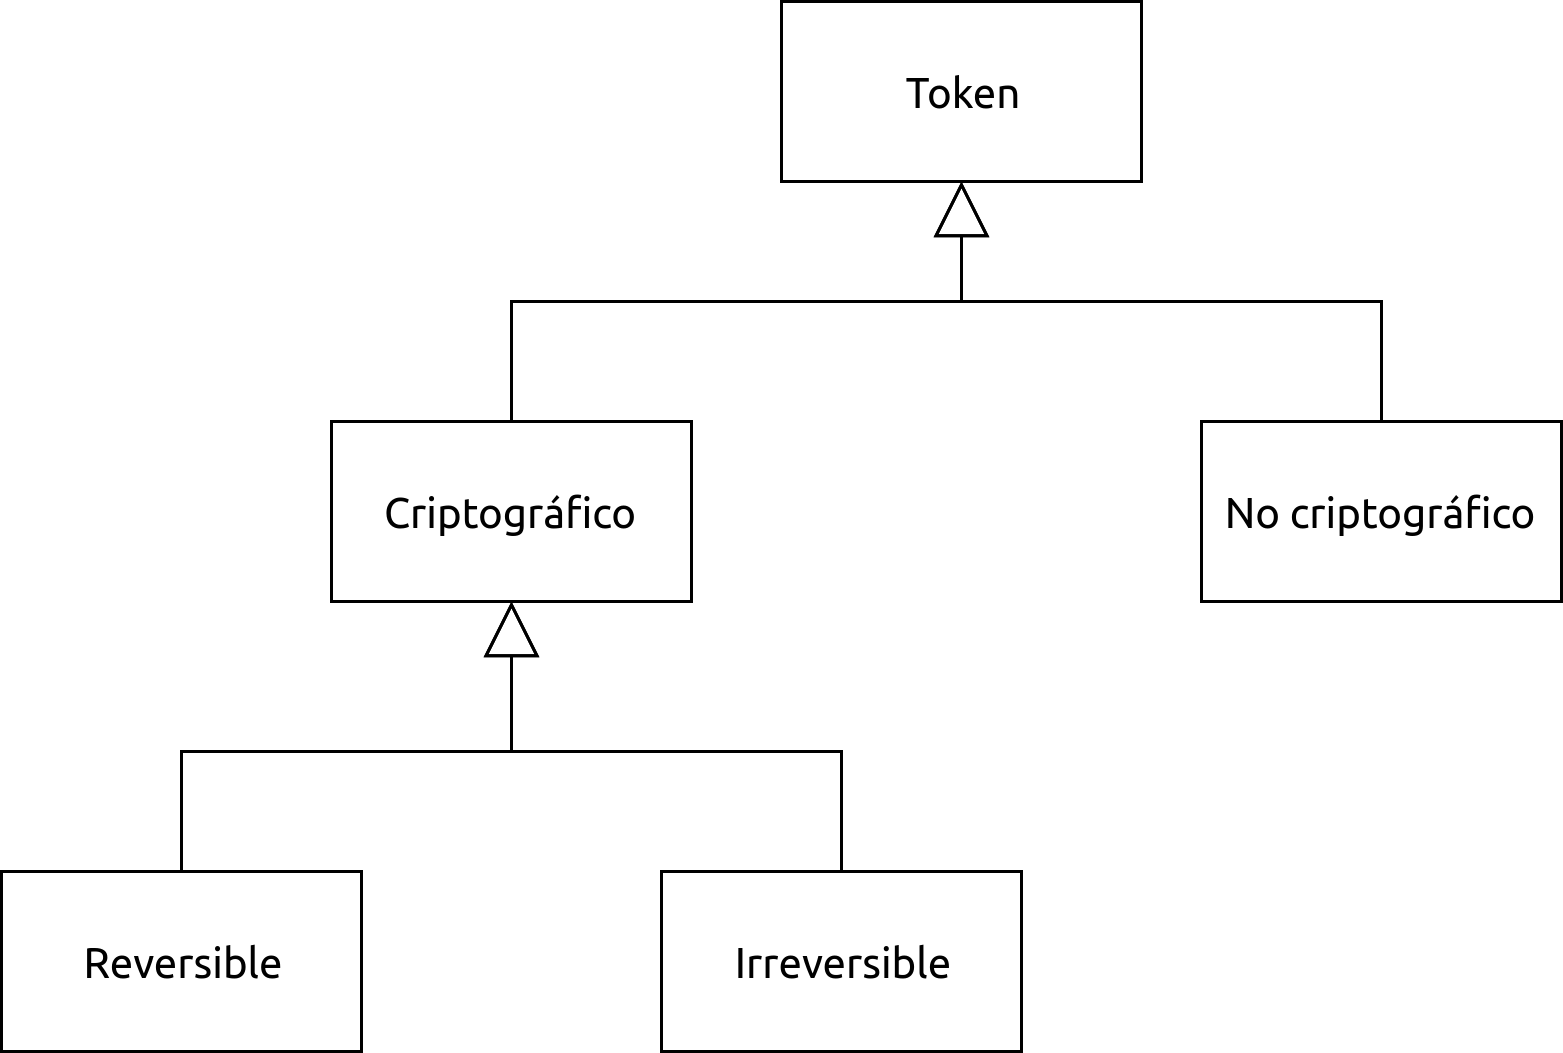
\includegraphics[width=0.75\linewidth]
        {../../../diagramas_comunes/clasificacion/clasificacion_propia.png}
      \caption{Clasificación propuesta.}
    \end{center}
  \end{figure}

  \note
  {
    Los únicos que se contemplan como «no criptográficos» son los que
    están basados en generadores realmente aleatorios. Todos los demás
    caen en la categoría de «criptográficos». Los reversibles son los que
    están basados en esquemas tradicionales (v. gr. los cifrados que
    preservan el formato). Los irreversibles necesitan de una base de datos
    para poder hacer el proceso inverso.
  }

\end{frame}
